\chapter{Strategy}
\section{Intento}

Ogni volta che si ha un algoritmo che ammette varianti si deve usare una Strategy, in moda da riutilizzare sempre lo stesso metodo (utile per aggiungere algoritmi in runtime).


%---
\section{Struttura}

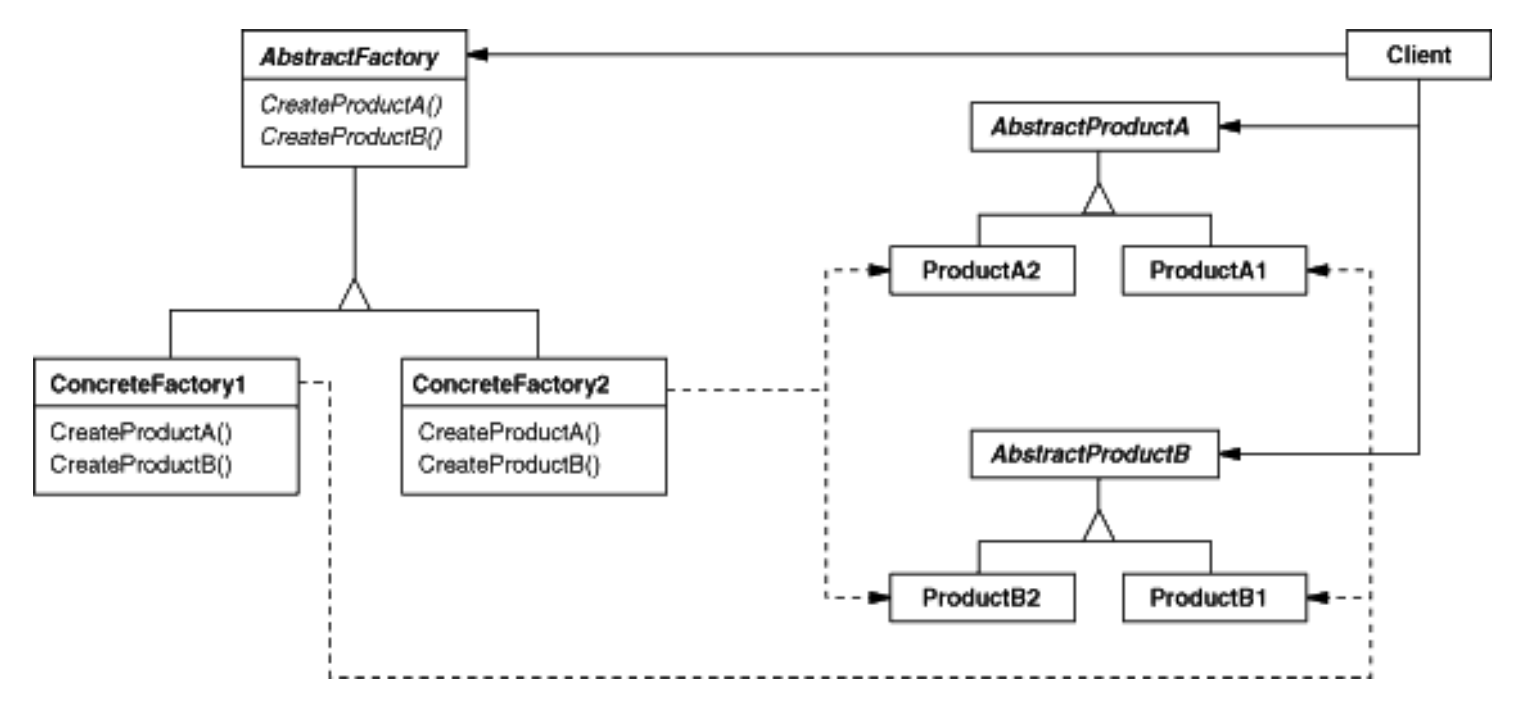
\includegraphics[width=\textwidth]{/Users/matt/Documents/GitHub/Design-Pattern-ITA/Strategy/Structure1}


%---
\section{Implementazione}

\subsection{Definizione delle interfacce Strategy e Context.}
Le interfacce Strategy e Context devono fornire a ConcreteStrategy l'accesso ai dati di cui ha bisogno.

Un approccio è fare in modo che Context passi i dati nei parametri a StrategyOperations.

In ogni caso, la Stategy può richiedere esattamente ciò di cui ha bisogno. Le esigenze del particolare algoritmo ed i suoi requisiti di dati determineranno la tecnica migliore.

\subsection{Rendere opzionali gli oggetti Strategy.}
La classe Context può essere semplificata se è significativo non avere un oggetto Strategy. Il Context controlla se ha uno StrategyObject prima di accedervi.

\begin{itemize}
    \item Se ce n'è uno, il Context lo usa normalmente.

    \item Se non c'è una Strategy, il contesto esegue il comportamento predefinito.
\end{itemize}

Il vantaggio di questo approccio è che i client non devono occuparsi affatto degli oggetti Strategy a meno che non amino il comportamento predefinito.


%---
\section{Esempio Java}
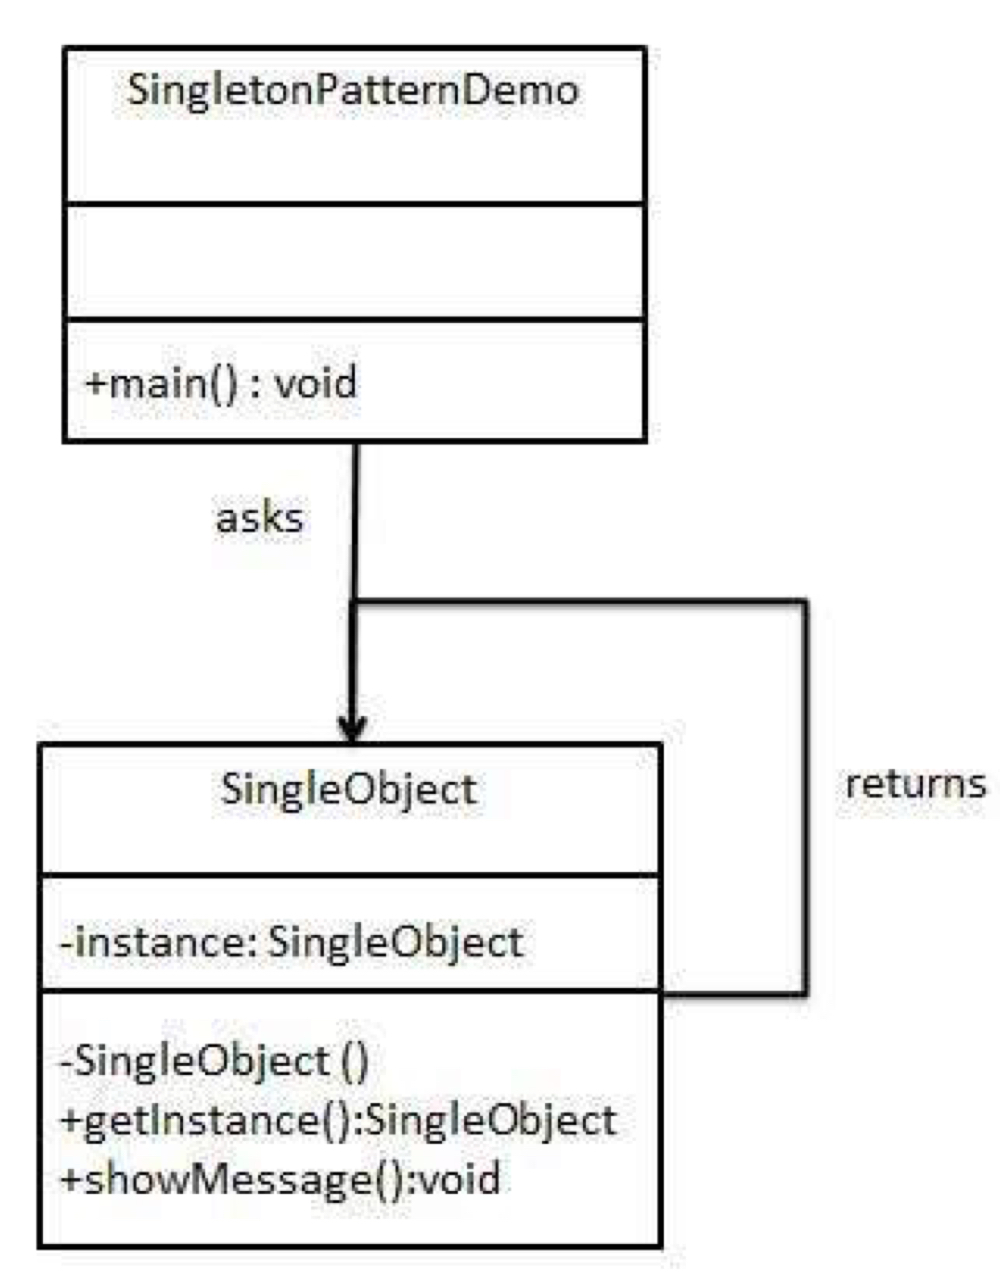
\includegraphics[width=\textwidth]{/Users/matt/Documents/GitHub/Design-Pattern-ITA/Strategy/Example1}

\subsection{Strategy.java}
\begin{lstlisting}[language=java]
    public interface Strategy {
        public int doOperation(int n1, int n2);
    }
\end{lstlisting}

\subsection{Context.java}
\begin{lstlisting}[language=java]
    public class Context {
        private Strategy strategy;
    
        public Context(Strategy strategy) {
            this.strategy = strategy;
        }
    
        public int executeStrategy(int n1, int n2) {
            return strategy.doOperation(n1, n2);
        }
    }
\end{lstlisting}

\subsection{OperationAdd.java}
\begin{lstlisting}[language=java]
    public class OperationAdd implements Strategy {

        @Override
        public int doOperation(int n1, int n2) {
            return n1 + n2;
        }
        
    }
\end{lstlisting}

\subsection{OperationMult.java}
\begin{lstlisting}[language=java]
    public class OperationMult implements Strategy {

        @Override
        public int doOperation(int n1, int n2) {
            return n1 * n2;
        }
        
    }
\end{lstlisting}

\subsection{main}
\begin{lstlisting}[language=java]
    public static void main(String[] args) {
        Context c;
        
        c = new Context(new OperationAdd());
        System.out.println("10 + 5 = " + c.executeStrategy(10, 5));
    
        c = new Context(new OperationMult());
        System.out.println("10 * 5 = " + c.executeStrategy(10, 5));
    }
\end{lstlisting}